\section{Introduction}
Time series data widely exist in real-world cyber-physical systems from transportation, finance, healthcare, weather, and other domains~\citep{qiu2024tfb,qiu2025tab,li2025TSFM-Bench}. Analyzing such time series data can lead to deep insights into the inherent dynamics, and boost decision-making in downstream tasks~\citep{qiu2025duet,wu2025k2vae,wu2024catch,wu2025srsnet,FOTraj}. In conventional pipelines, data scientists play a vital role in process orchestration and model design. Though facilitating the promotion of time series analysis, they heavily rely on expert prior knowledge and lack automation. To explore a fully-agentic paradigm which can work as smartly as human experts, recent studies focus on unleashing the potential of LLMs in time series analysis through constructing reasoning corpus, covering analytical tasks and reasoning tasks~\citep{TimeMQA,cai2024timeseriesexam}, and then training Time Series Reasoning Models (TSRMs) on them~\citep{xie2024chatts,zhou2025merit,sui2025training}. However, there still remain some limitations in TSRMs, making them struggle to replace data scientists.

\begin{figure}[t]
    \centering
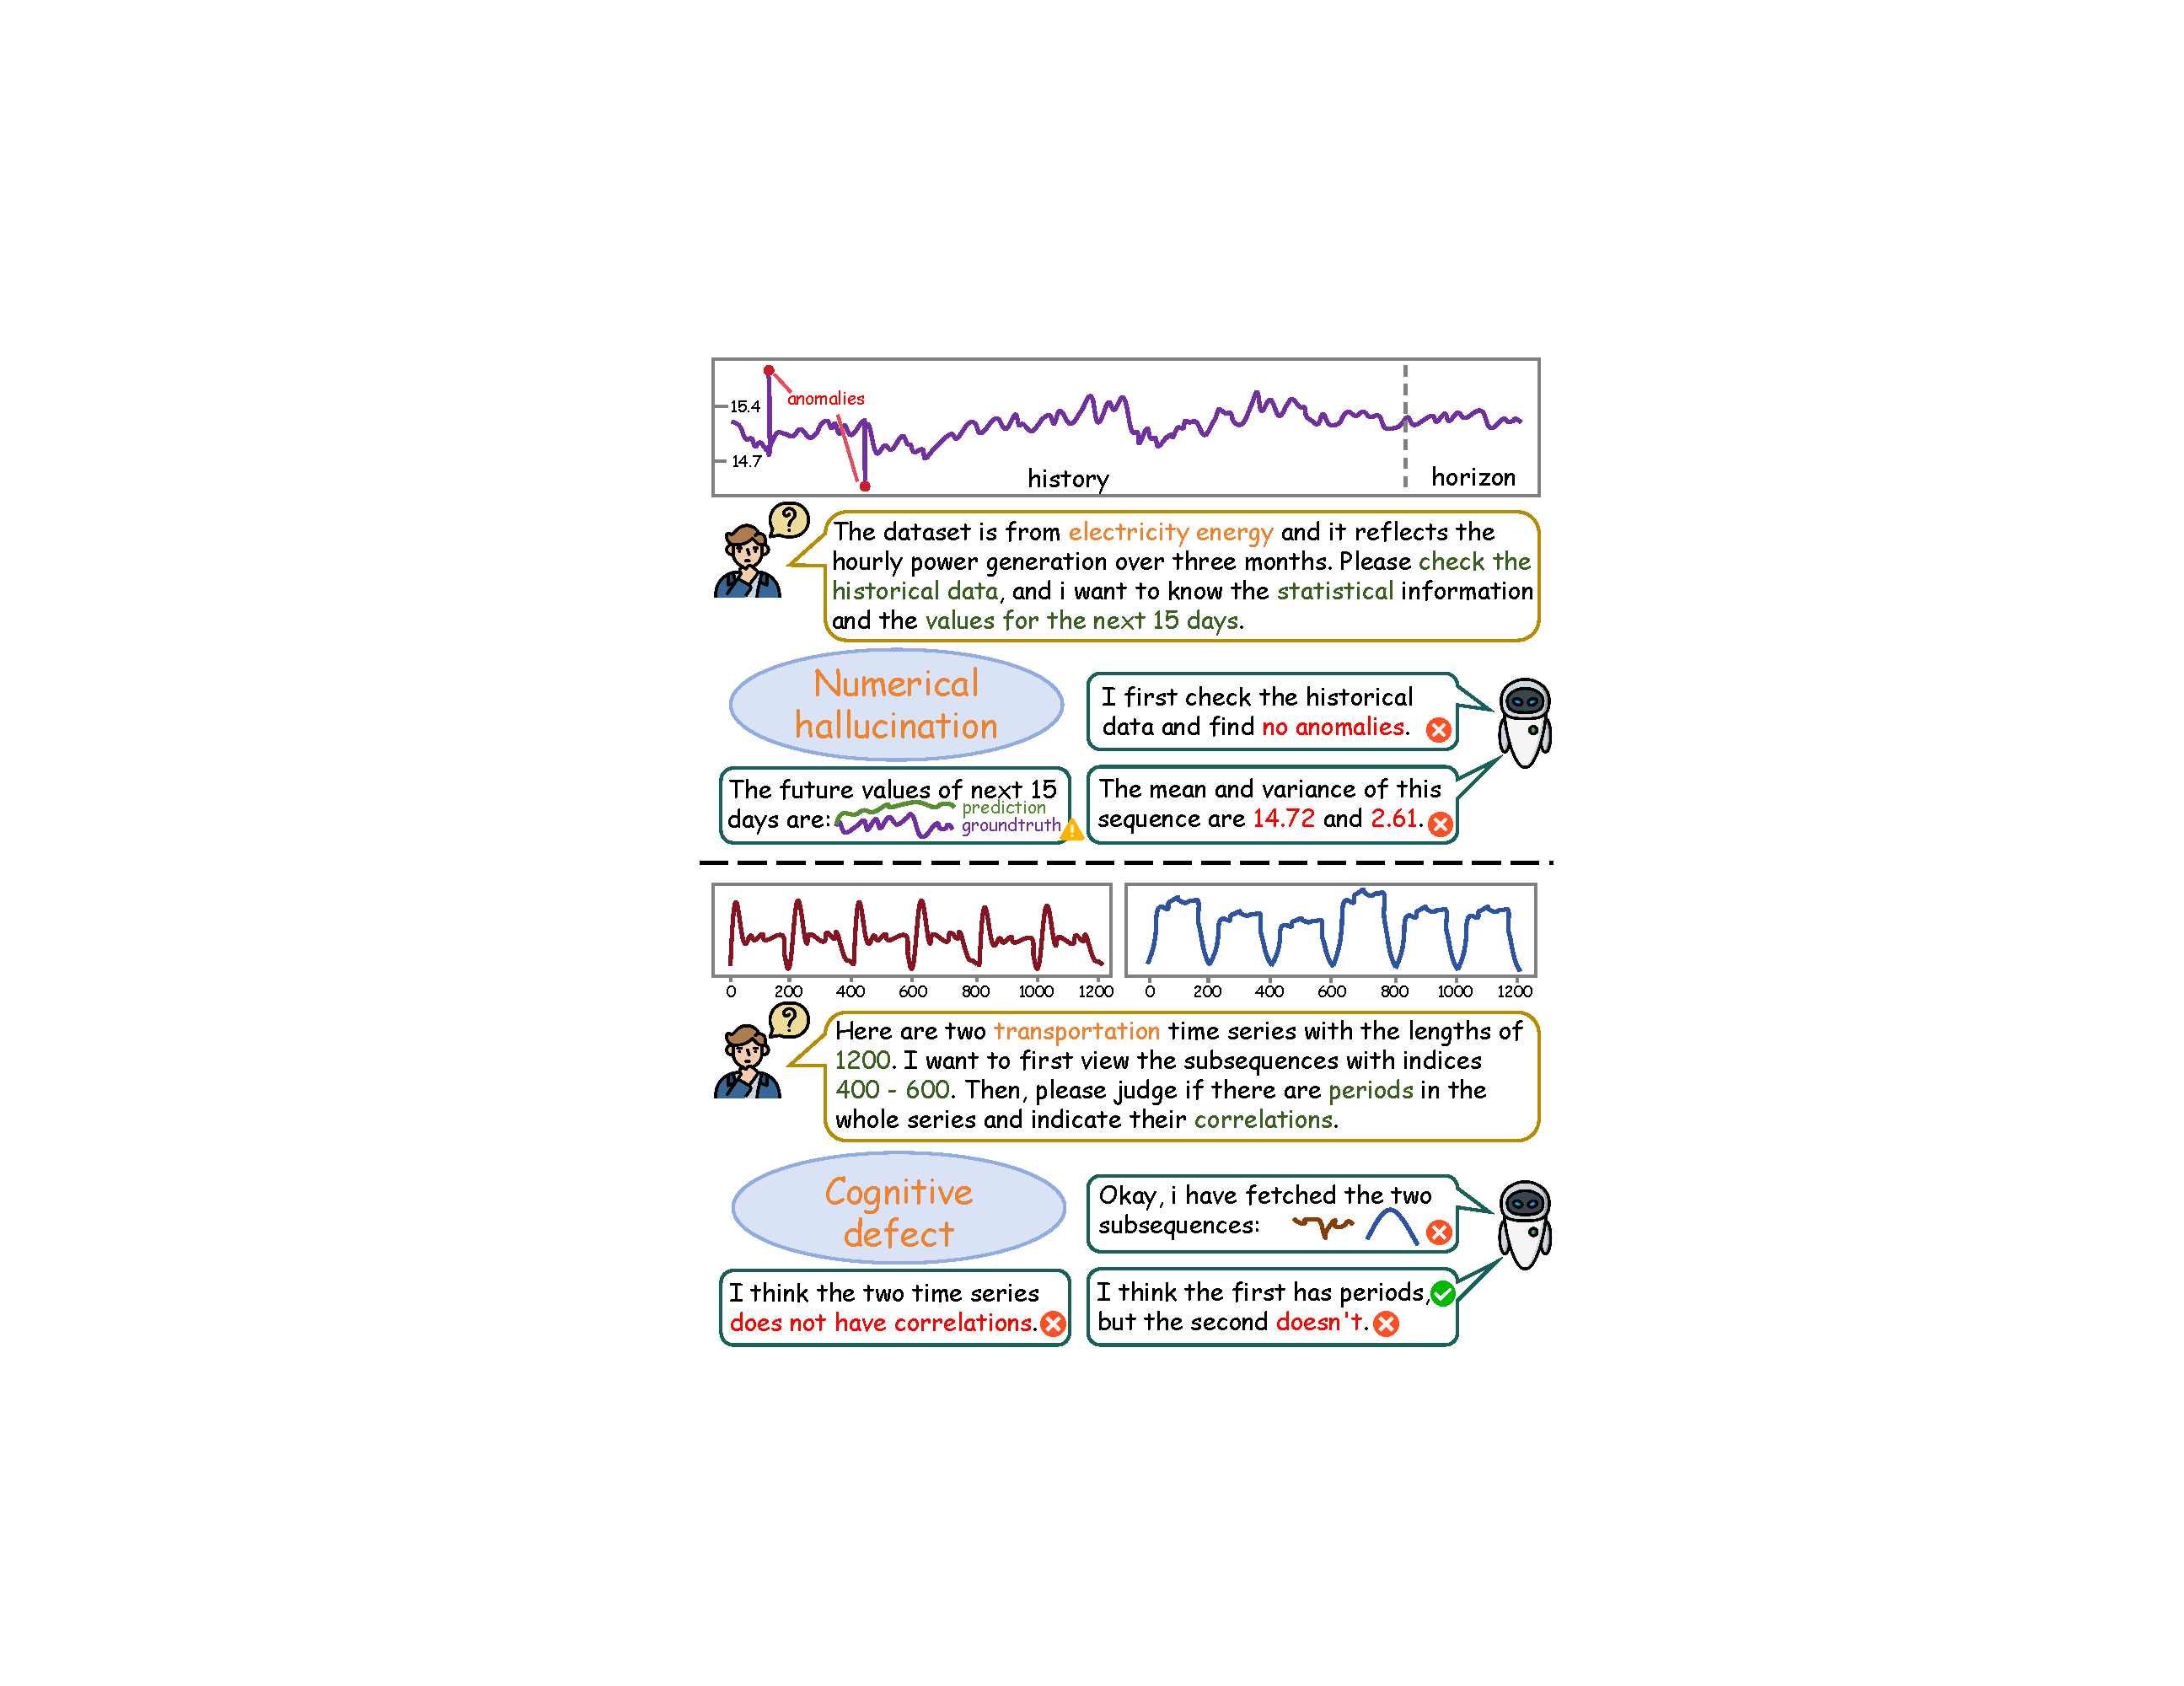
\includegraphics[width=0.92\linewidth]{Figures/intro1.pdf}
    \caption{Common dilemmas in time series reasoning, i.e., \textit{numerical hallucination} and \textit{cognitive defect}.}
\label{fig: intro1}
\end{figure}

Current studies on TSRMs~\citep{xie2024chatts,TimeMQA} aim to strengthen and unleash the inherent capabilities of LLMs in time series reasoning tasks, which requires LLMs to fully understand the internal connections of structured numerical values. Due to the discrete tokenization of LLMs, they often struggle to handle such numerical tasks and prove suboptimal in analytical tasks like forecasting~\citep{tan2024language} and anomaly detection~\citep{zhou2024can}. In reasoning tasks, they also face two main problems in processing time series data--see Figure~\ref{fig: intro1}: 1) \textit{numerical hallucination}. TSRMs cannot accurately understand and calculate statistical characteristics of time series, nor make reliable forecasts and anomaly detections; 2) \textit{cognitive defect}. When the input time series is long, and the questions are flexible and complex, TSRMs struggle to provide correct analytics. From our perspective, \textit{simulating data scientists with TSRMs but not providing strong analytical tools they often use} does hinder the capabilities.

\begin{figure}[t]
    \centering
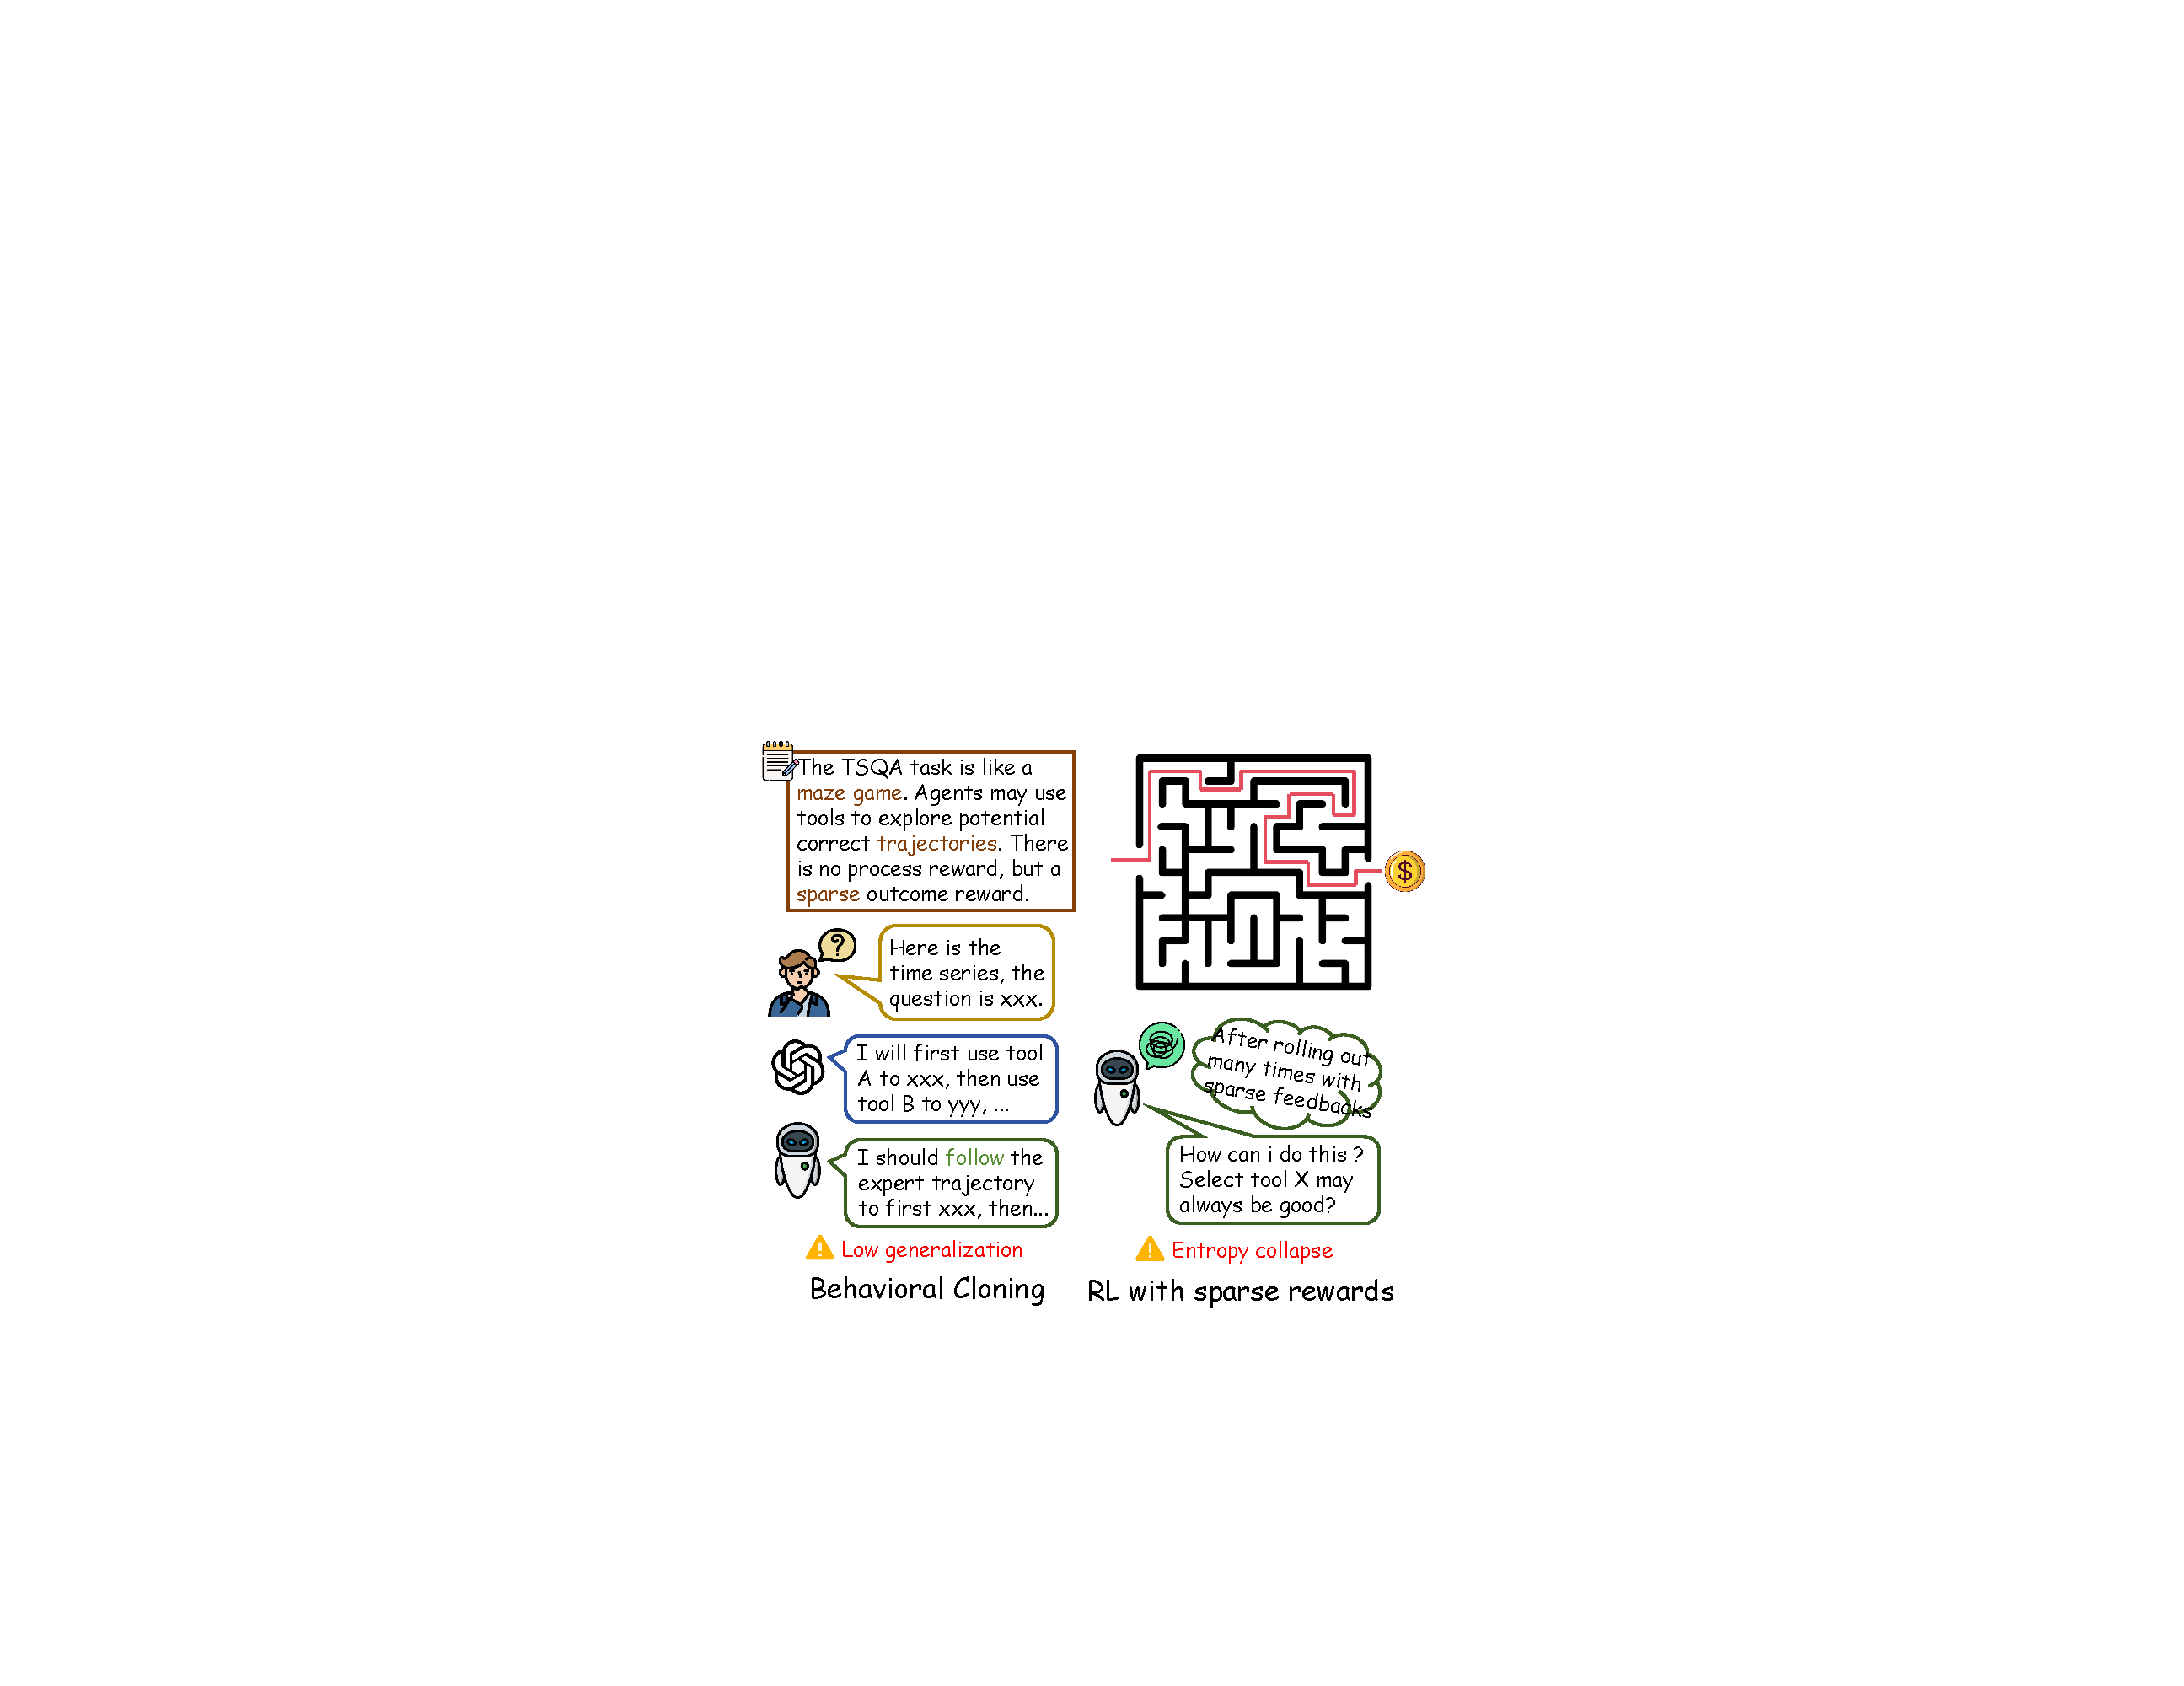
\includegraphics[width=0.82\linewidth]{Figures/intro2.pdf}
    \caption{Common dilemmas in behaviour cloning and reinforcement learning, causing \textit{low generalization} and \textit{entropy collapse}.}
\label{fig: intro2}
\end{figure}

To overcome the above-mentioned problems, we propose \textbf{TimeART}, a \textbf{\underline{Time}} series \textbf{\underline{A}}gentic \textbf{\underline{R}}easoning framework with \textbf{\underline{T}}ool-augmentation. It integrates \textit{21} strong out-of-the-box tools for time series analysis, which include statistical methods to lightweight time series foundation models~\citep{wang2025lightgts,shentu2024towards}, allowing TSRMs to autonomously, robustly, and efficiently use tools in the reasoning process. Furthermore, in order to strengthen the tool invocation capability of TSRMs, we propose \textbf{TimeToolBench}, a comprehensive corpus for agentic time series reasoning, containing \textit{100k} ReAct-style~\citep{yao2022react} tool-use trajectories from multiple real-world domains, collected with GPT-4o and valiated through a strict scheme. This provides a general solution to finetune any open-source LLM with this corpus to strong TSRM supporting tool-use.

On the other hand, the training paradigm of TSRMs with tool-use also matters. Current training paradigm from other domains, e.g. math reasoning agent~\citep{forootani2025survey}, GUI agent~\citep{zhang2024large}, and web agent~\citep{ning2025survey}, mainly adopts first behaviour cloning then reinforcement learning. In these domains, the extent of behaviour cloning is widely studied and the process reward of reinforcement learning is clearly-defined. However, this paradigm faces some challenges in time series reasoning--see Figure~\ref{fig: intro2}: 1) \textit{low generalization.} The balance of behaviour cloning is hard to control, often causing TSRMs to simply imitate the tool-use trajectories of experts. 2) \textit{entropy collapse.} The reward of reinforcement learning in time series reasoning tasks is sparse, lacking the process reward and only possessing the outcome reward. This makes TSRMs hard to understand the environment (world modeling) and tend to output conservative decisions.

The underlying principle of agentic reinforcement learning~\citep{zhang2509landscape} is to implicitly align the preferences of the reward functions with the model, allowing it to model the endogenous world for preference-based decision-making. However, it is limited by the design of reward functions and quality of rollouts, especially when the reward is sparse. To tackle this, we draw inspiration from experience learning~\citep{zhang2025agent,fang2025play2prompt,tang2025chemagent}, and first devise multiple stages to train the TSRMs for agentic reasoning, which allows them to learn from early exploration experience and self-reflection. The training strategy boosts perceiving the action space and the external environment, learning the strategic tool-use, and understanding the underlying principles. It functionally replaces conventional (SFT + RL) process and is easier to train, which are experimentally demonstrated in Section~\ref{sec: model analysis}, thus enhancing the generalization and robustness in endowing TSRMs with the capability to invoke proper tools according to scenarios.

Our contributions are summarized as:

\begin{itemize}[left=0.1cm]
\item We introduce \textbf{TimeART}, an Agentic Time Series Reasoning framework supporting tool-use. It integrates \textit{21} strong out-of-the-box analytical tools, allowing TSRMs to autonomously, robustly, and efficiently invoke them during reasoning. TSRMs can be further strengthened through training on the proposed \textbf{TimeToolBench}, a corpus containing \textit{100k} high-quality tool-use trajectories.

\item We devise a novel training strategy to mitigate the dilemmas in conventional paradigms. It decomposes the underlying principles of agentic reinforcement learning into several parts, enabling the TSRMs to better perceive the external environment and the action space, thus preserving the generalization capability. 

\item Experimentally, we train an 8B TSRM on \textbf{TimeToolBench} through our proposed training strategy, and then equip it with the \textbf{TimeART} framework. It is demonstrated state-of-the-art performance on multiple TSQA benchmarks. 

\end{itemize}